\chapter{Implementation}
\label{chapter:5}

The first step to implement interoperability through the Diaspora
protocol is to offer a mechanism to discover and provide users and
public profiles, in this case using WebFinger and hCard.

The second step is to implement a message exchange mechanism to provide
the means to talk to third-party servers. The Diaspora protocol proposes
the exchange of messages containing entities that represent contents and
interactions. For now, Noosfero should handle the following entities:

\begin{itemize}
  \item Profiles creation, update, and removal
  \item Publications and comments creation and removal
  \item Content subscriptions and unsubscriptions
  \item User relationships (follow and unfollow)
\end{itemize}

The following sections also describe technical specifications of the
Diaspora protocol, and could be used as reference for future
implementations.

\section{User Discovery}

The Diaspora protocol proposes the use of WebFinger to fetch user
identities and hCard to share public profiles. The implementation used
in the Diaspora project still uses XML to format WebFinger payloads,
what is considered legacy.

\begin{figure}[h]
	\centering
		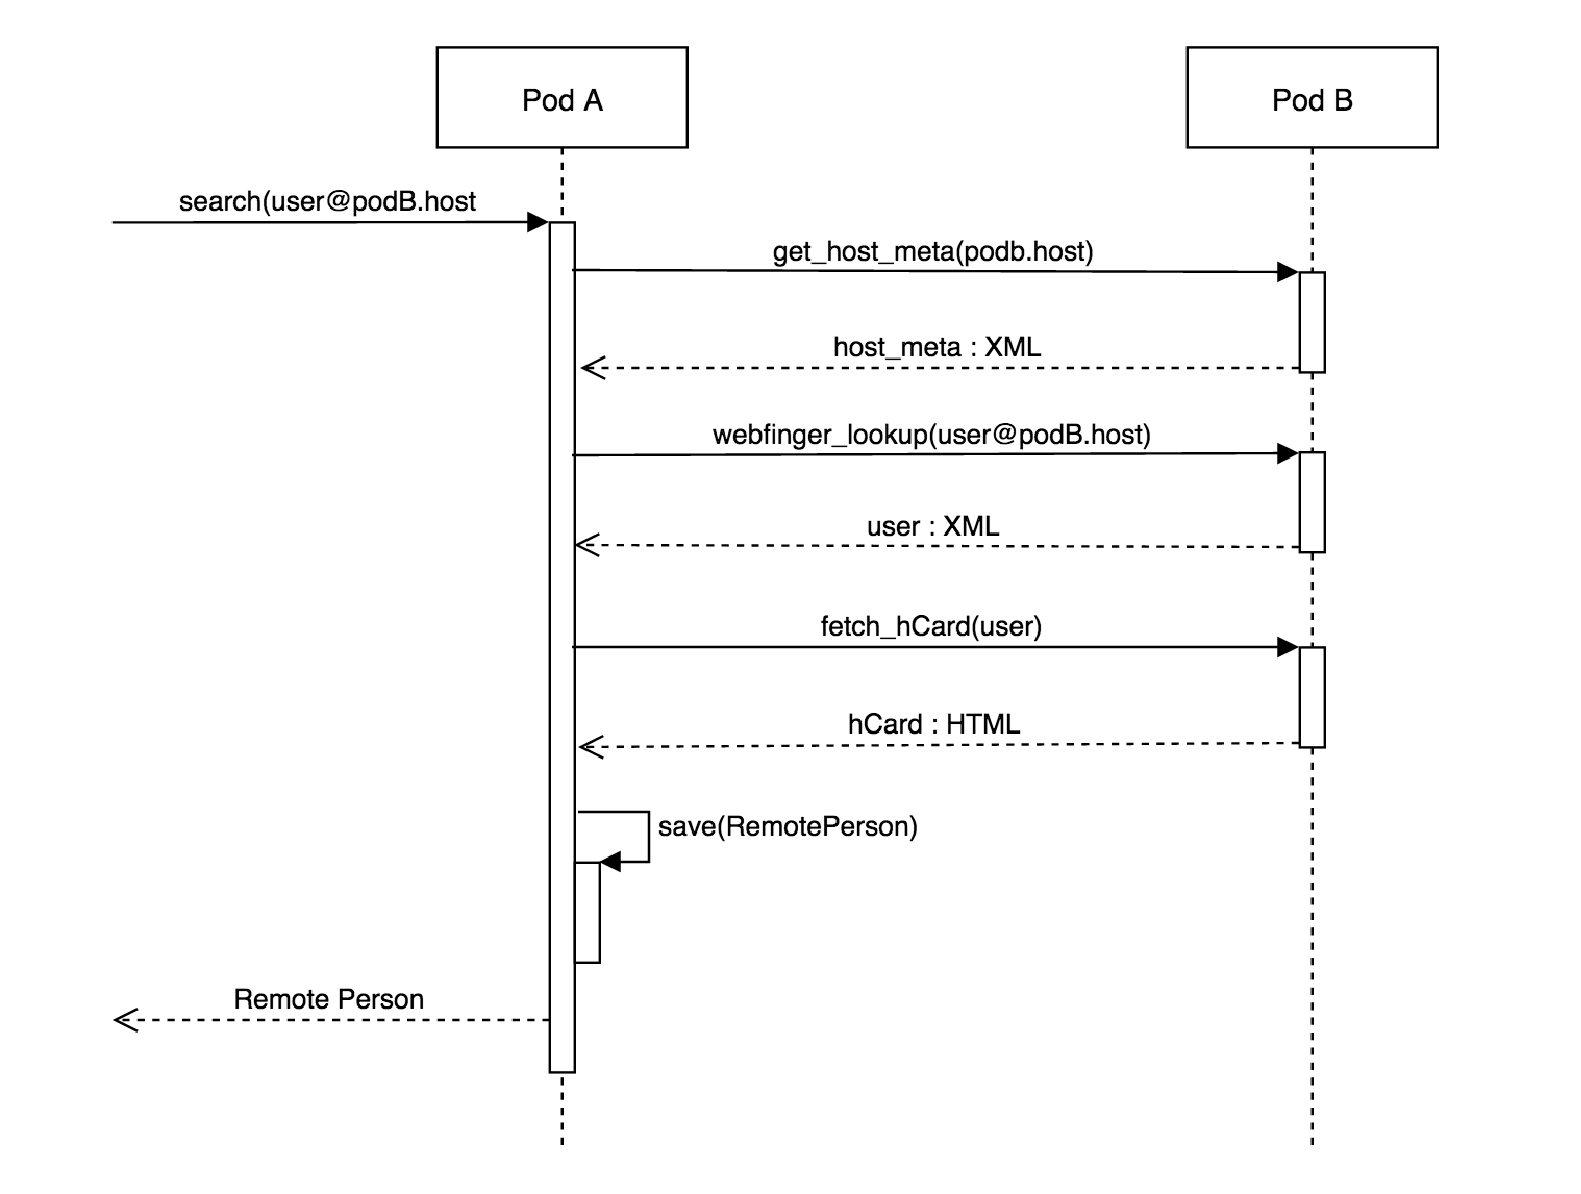
\includegraphics[width=0.5\textwidth]{figures/seq_descoberta.eps}
	\caption{Sequence diagram of the user discovery process}
	\label{fig:seq_discovery}
\end{figure}

The discovery process is described in Figure \ref{fig:seq_discovery},
where the remote server is queried with an identifier in the format
\textit{user@host}. The discovery endpoint can be found in the server
metadata, also obtained via WebFinger, on a standard endpoint. After the
identity lookup, the remote server is queried again for the public
profile, which in turn is obtained via hCard in HTML format.

As the discovery implementation is based on WebFinger, it is possible to
find users on any application that responds to this format.

\section{Message Exchange}

To follow an external user, it is necessary to send a private Salmon
message to its endpoint. Receiving the message, the Diaspora server
creates a local profile to represent the remote user locally --- only
after querying the Noosfero server for its server metadata and the
user's public profile. This process is shown in Figure
\ref{fig:seq_contact}, and includes part of the discovery process.

\begin{figure}[h]
	\centering
		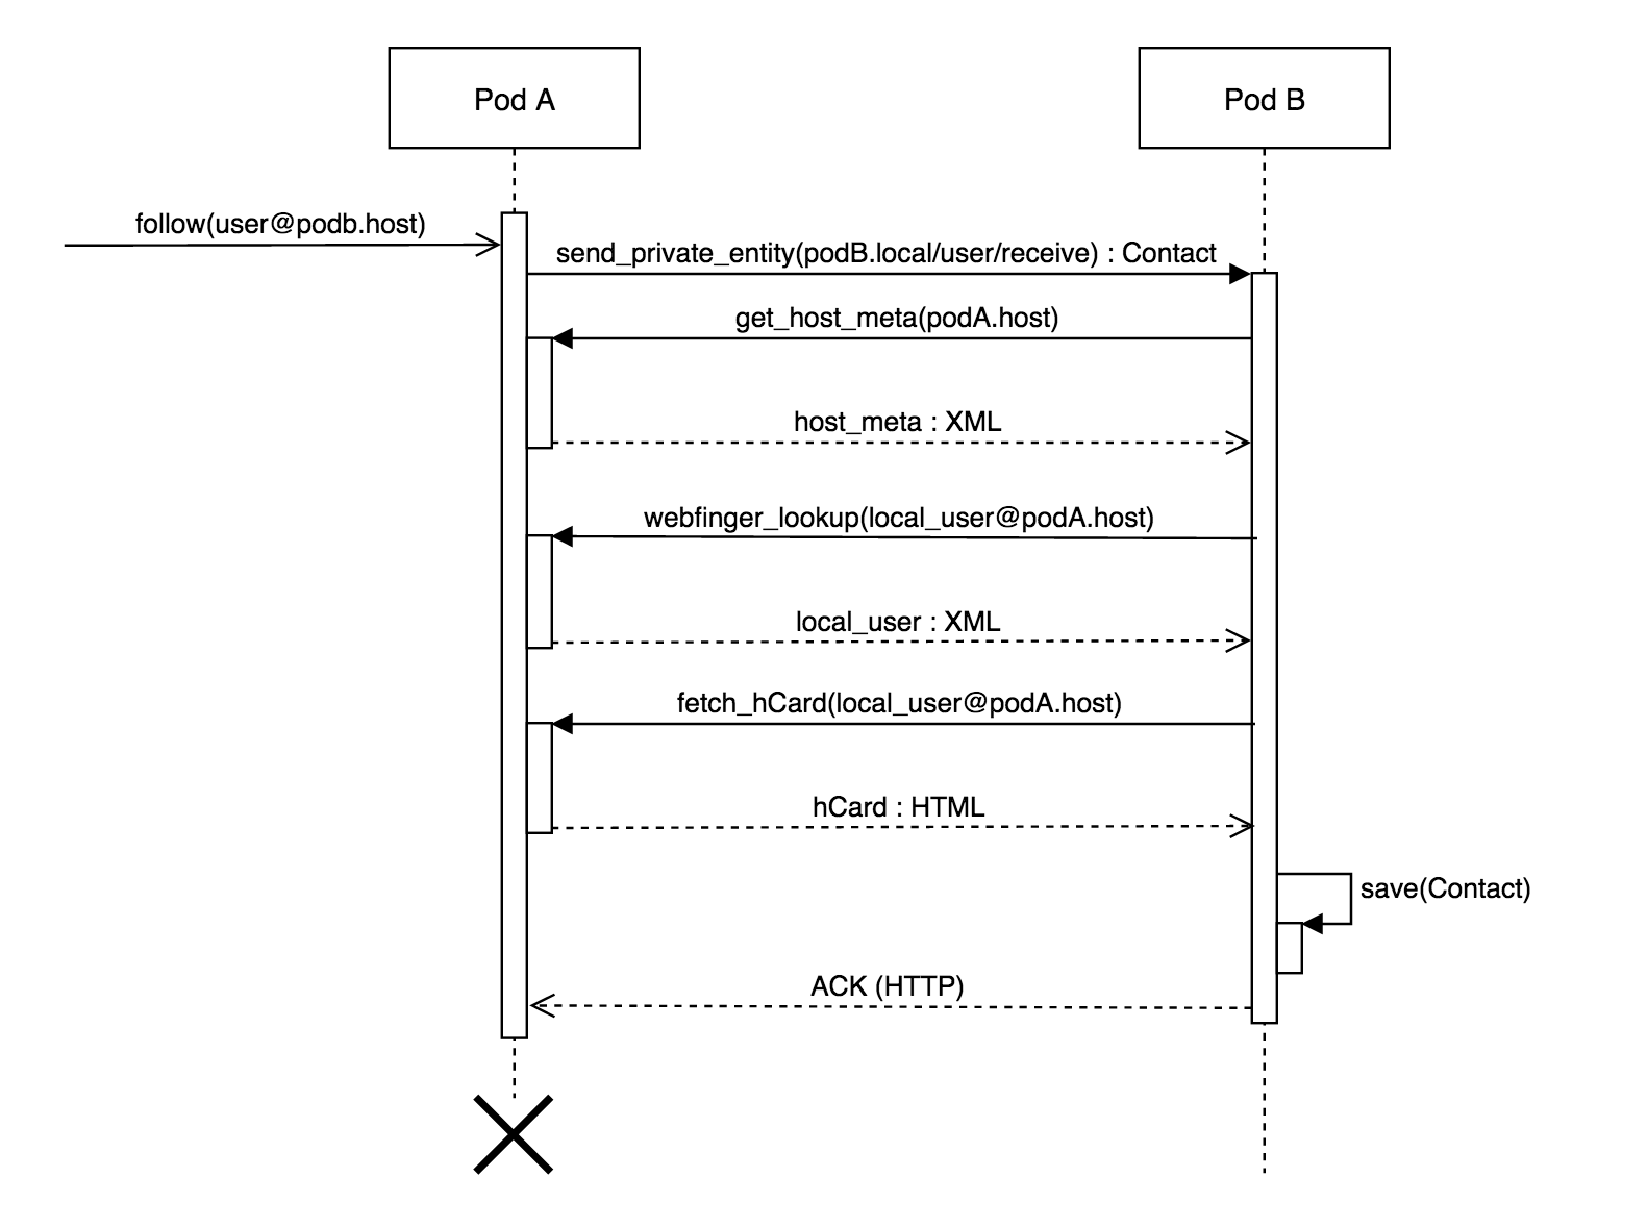
\includegraphics[width=0.5\textwidth]{figures/seq_contato.eps}
	\caption{Sequence diagram of the contacts sharing process}
	\label{fig:seq_contact}
\end{figure}

It is crucial to make sure that the message was successfully delivered,
otherwise the servers will not share the same state. The server sending
the message should offer some kind of reliability, retrying or even
undoing actions when facing communication problems. When trying to
follow a remote user, Noosfero will retry a predefined number of times,
and then destroy the relationship locally if the remote server did not
respond with a success status.

Private salmon messages are encrypted with RSA to ensure
confidentiality, which requires every user to have a pair of RSA keys.
The proposed implementation for Noosfero uses the OpenSSL Ruby bindings
to generate a key pair for every user, as soon as that is necessary.

The last step is to handle incoming entities representing user contents.
As shown in Figure \ref{fig:seq_publication}, new contents are sent by
Diaspora to every server that is involved in the interaction --- in this
case, the origin of users following the author of the new content. At
the time of writing, Noosfero supports only public content.

\begin{figure}[h]
	\centering
		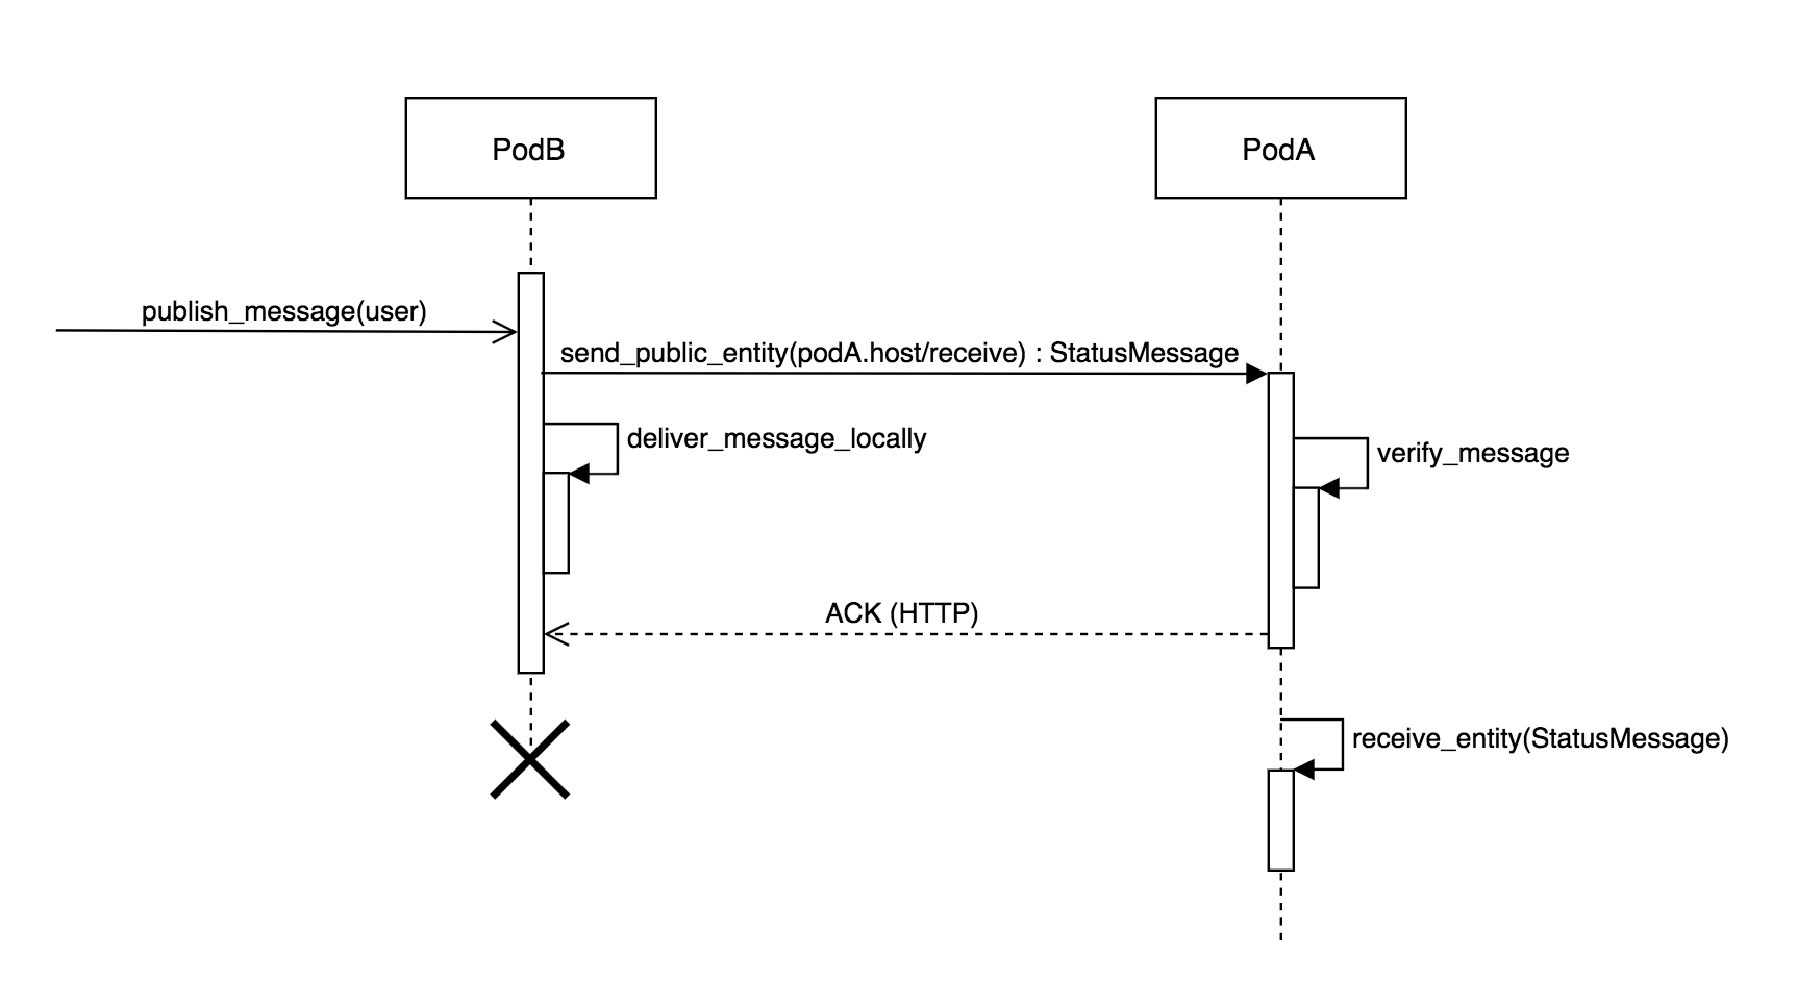
\includegraphics[width=0.5\textwidth]{figures/seq_publicacao.eps}
	\caption{Sequence diagram of the publication sending process}
	\label{fig:seq_publication}
\end{figure}

After receiving the publication notification in a public Salmon message,
Noosfero  saves the data locally. It is also necessary to include a GUID
(Globally Unique IDentifier), required as identifier for all entities sent
across servers.

It is also important to handle retraction entities to maintain the same state
in all servers. These entities are sent every time a content or user profile is
removed, and have the same visibility as the original content.  Handling a
retraction involves querying for a related local entity that matches the one
that has been removed remotely, so that the removal can be replicated locally.
